\batchmode
\documentclass[twoside]{book}

% Packages required by doxygen
\usepackage{fixltx2e}
\usepackage{calc}
\usepackage{doxygen}
\usepackage[export]{adjustbox} % also loads graphicx
\usepackage{graphicx}
\usepackage[utf8]{inputenc}
\usepackage{makeidx}
\usepackage{multicol}
\usepackage{multirow}
\PassOptionsToPackage{warn}{textcomp}
\usepackage{textcomp}
\usepackage[nointegrals]{wasysym}
\usepackage[table]{xcolor}

% Font selection
\usepackage[T1]{fontenc}
\usepackage[scaled=.90]{helvet}
\usepackage{courier}
\usepackage{amssymb}
\usepackage{sectsty}
\renewcommand{\familydefault}{\sfdefault}
\allsectionsfont{%
  \fontseries{bc}\selectfont%
  \color{darkgray}%
}
\renewcommand{\DoxyLabelFont}{%
  \fontseries{bc}\selectfont%
  \color{darkgray}%
}
\newcommand{\+}{\discretionary{\mbox{\scriptsize$\hookleftarrow$}}{}{}}

% Page & text layout
\usepackage{geometry}
\geometry{%
  a4paper,%
  top=2.5cm,%
  bottom=2.5cm,%
  left=2.5cm,%
  right=2.5cm%
}
\tolerance=750
\hfuzz=15pt
\hbadness=750
\setlength{\emergencystretch}{15pt}
\setlength{\parindent}{0cm}
\setlength{\parskip}{3ex plus 2ex minus 2ex}
\makeatletter
\renewcommand{\paragraph}{%
  \@startsection{paragraph}{4}{0ex}{-1.0ex}{1.0ex}{%
    \normalfont\normalsize\bfseries\SS@parafont%
  }%
}
\renewcommand{\subparagraph}{%
  \@startsection{subparagraph}{5}{0ex}{-1.0ex}{1.0ex}{%
    \normalfont\normalsize\bfseries\SS@subparafont%
  }%
}
\makeatother

% Headers & footers
\usepackage{fancyhdr}
\pagestyle{fancyplain}
\fancyhead[LE]{\fancyplain{}{\bfseries\thepage}}
\fancyhead[CE]{\fancyplain{}{}}
\fancyhead[RE]{\fancyplain{}{\bfseries\leftmark}}
\fancyhead[LO]{\fancyplain{}{\bfseries\rightmark}}
\fancyhead[CO]{\fancyplain{}{}}
\fancyhead[RO]{\fancyplain{}{\bfseries\thepage}}
\fancyfoot[LE]{\fancyplain{}{}}
\fancyfoot[CE]{\fancyplain{}{}}
\fancyfoot[RE]{\fancyplain{}{\bfseries\scriptsize Generated by Doxygen }}
\fancyfoot[LO]{\fancyplain{}{\bfseries\scriptsize Generated by Doxygen }}
\fancyfoot[CO]{\fancyplain{}{}}
\fancyfoot[RO]{\fancyplain{}{}}
\renewcommand{\footrulewidth}{0.4pt}
\renewcommand{\chaptermark}[1]{%
  \markboth{#1}{}%
}
\renewcommand{\sectionmark}[1]{%
  \markright{\thesection\ #1}%
}

% Indices & bibliography
\usepackage{natbib}
\usepackage[titles]{tocloft}
\setcounter{tocdepth}{3}
\setcounter{secnumdepth}{5}
\makeindex

% Hyperlinks (required, but should be loaded last)
\usepackage{ifpdf}
\ifpdf
  \usepackage[pdftex,pagebackref=true]{hyperref}
\else
  \usepackage[ps2pdf,pagebackref=true]{hyperref}
\fi
\hypersetup{%
  colorlinks=true,%
  linkcolor=blue,%
  citecolor=blue,%
  unicode%
}

% Custom commands
\newcommand{\clearemptydoublepage}{%
  \newpage{\pagestyle{empty}\cleardoublepage}%
}

\usepackage{caption}
\captionsetup{labelsep=space,justification=centering,font={bf},singlelinecheck=off,skip=4pt,position=top}

%===== C O N T E N T S =====

\begin{document}

% Titlepage & ToC
\hypersetup{pageanchor=false,
             bookmarksnumbered=true
            }
\pagenumbering{alph}
\pagenumbering{arabic}
\hypersetup{pageanchor=true}

%--- Begin generated contents ---
\chapter{Demo problem\+: Fluid Mechanics on unstructured meshes}
\label{index}\hypertarget{index}{}\hypertarget{index_q}{}\section{A few quick questions...}\label{index_q}
Since {\ttfamily oomph-\/lib} is developed as open-\/source software, any evidence that the code is being downloaded and used is very helpful for us as it helps to justify our continued work on this project.

We would therefore be extremely grateful if you could provide the information requested in the form below. Pressing the \char`\"{}submit\char`\"{} button will get you to the actual download page.

{\bfseries Note\+:} 
\begin{DoxyItemize}
\item All information will be treated as confidential. 
\item If you provide your email address and check the appropriate box we will add you to our mailing list to inform you of upgrades and bug fixes to the code. Rest assured that the mailing list is {\bfseries very low volume} -- we have better things to do than to bombard you with email. 
\item If you still feel reluctant to provide any of the information requested, feel free to enter some dummy input. The form will check that {\bfseries some} information has been entered but entering your name as \char`\"{}\+Joe Cool\char`\"{} is perfectly acceptable -- this is to discourage people from not providing the information simply because they are too lazy to type... 
\end{DoxyItemize}



 







 

 \hypertarget{index_pdf}{}\section{P\+D\+F file}\label{index_pdf}
A \href{../latex/refman.pdf}{\tt pdf version} of this document is available. \end{document}

\chapter{Namespace Index}
\section{Namespace List}
Here is a list of all namespaces with brief descriptions\+:\begin{DoxyCompactList}
\item\contentsline{section}{\hyperlink{namespaceGlobal__Physical__Variables}{Global\+\_\+\+Physical\+\_\+\+Variables} \\*Global variables that represent physical properties }{\pageref{namespaceGlobal__Physical__Variables}}{}
\item\contentsline{section}{\hyperlink{namespaceoomph}{oomph} }{\pageref{namespaceoomph}}{}
\item\contentsline{section}{\hyperlink{namespacePhysical__Variables}{Physical\+\_\+\+Variables} \\*Namespace for the solution of 2D linear shell equation }{\pageref{namespacePhysical__Variables}}{}
\end{DoxyCompactList}

\chapter{Hierarchical Index}
\section{Class Hierarchy}
This inheritance list is sorted roughly, but not completely, alphabetically\+:\begin{DoxyCompactList}
\item Problem\begin{DoxyCompactList}
\item \contentsline{section}{Unstructured\+Solid\+Problem$<$ E\+L\+E\+M\+E\+NT $>$}{\pageref{classUnstructuredSolidProblem}}{}
\end{DoxyCompactList}
\end{DoxyCompactList}

\chapter{Class Index}
\section{Class List}
Here are the classes, structs, unions and interfaces with brief descriptions\+:\begin{DoxyCompactList}
\item\contentsline{section}{\hyperlink{classPMLProblem}{P\+M\+L\+Problem$<$ E\+L\+E\+M\+E\+N\+T $>$} }{\pageref{classPMLProblem}}{}
\item\contentsline{section}{\hyperlink{classGlobalParameters_1_1TestPMLMapping}{Global\+Parameters\+::\+Test\+P\+M\+L\+Mapping} }{\pageref{classGlobalParameters_1_1TestPMLMapping}}{}
\end{DoxyCompactList}

\chapter{File Index}
\section{File List}
Here is a list of all files with brief descriptions\+:\begin{DoxyCompactList}
\item\contentsline{section}{\hyperlink{jeffery__orbit_8cc}{jeffery\+\_\+orbit.\+cc} }{\pageref{jeffery__orbit_8cc}}{}
\item\contentsline{section}{\hyperlink{jeffery__orbit_8txt__doxygenified_8h}{jeffery\+\_\+orbit.\+txt\+\_\+doxygenified.\+h} }{\pageref{jeffery__orbit_8txt__doxygenified_8h}}{}
\item\contentsline{section}{\hyperlink{my__taylor__hood__elements_8h}{my\+\_\+taylor\+\_\+hood\+\_\+elements.\+h} }{\pageref{my__taylor__hood__elements_8h}}{}
\end{DoxyCompactList}

\chapter{Namespace Documentation}
\hypertarget{namespaceGlobal__Physical__Variables}{}\section{Global\+\_\+\+Physical\+\_\+\+Variables Namespace Reference}
\label{namespaceGlobal__Physical__Variables}\index{Global\+\_\+\+Physical\+\_\+\+Variables@{Global\+\_\+\+Physical\+\_\+\+Variables}}


Namespace for physical parameters.  


\subsection*{Functions}
\begin{DoxyCompactItemize}
\item 
Vector$<$ double $>$ \hyperlink{namespaceGlobal__Physical__Variables_afae321364975eb56688ad13abc8ed6b7}{Gravity} (2)
\begin{DoxyCompactList}\small\item\em Gravity vector. \end{DoxyCompactList}\item 
void \hyperlink{namespaceGlobal__Physical__Variables_a87da705b8a46bed337cf5dbdd788b87b}{body\+\_\+force} (const double \&time, const Vector$<$ double $>$ \&x, Vector$<$ double $>$ \&result)
\begin{DoxyCompactList}\small\item\em Functional body force. \end{DoxyCompactList}\item 
void \hyperlink{namespaceGlobal__Physical__Variables_a9780d615ae07c4e00a436ab2973b54e6}{zero\+\_\+body\+\_\+force} (const double \&time, const Vector$<$ double $>$ \&x, Vector$<$ double $>$ \&result)
\begin{DoxyCompactList}\small\item\em Zero functional body force. \end{DoxyCompactList}\end{DoxyCompactItemize}
\subsection*{Variables}
\begin{DoxyCompactItemize}
\item 
double \hyperlink{namespaceGlobal__Physical__Variables_ab814e627d2eb5bc50318879d19ab16b9}{Re} =100
\begin{DoxyCompactList}\small\item\em Reynolds number. \end{DoxyCompactList}\item 
double \hyperlink{namespaceGlobal__Physical__Variables_ab1a845a672b4d74b304639a976dc65c6}{Re\+\_\+inv\+Fr} =100
\begin{DoxyCompactList}\small\item\em Reynolds/\+Froude number. \end{DoxyCompactList}\end{DoxyCompactItemize}


\subsection{Detailed Description}
Namespace for physical parameters. 

\subsection{Function Documentation}
\mbox{\Hypertarget{namespaceGlobal__Physical__Variables_a87da705b8a46bed337cf5dbdd788b87b}\label{namespaceGlobal__Physical__Variables_a87da705b8a46bed337cf5dbdd788b87b}} 
\index{Global\+\_\+\+Physical\+\_\+\+Variables@{Global\+\_\+\+Physical\+\_\+\+Variables}!body\+\_\+force@{body\+\_\+force}}
\index{body\+\_\+force@{body\+\_\+force}!Global\+\_\+\+Physical\+\_\+\+Variables@{Global\+\_\+\+Physical\+\_\+\+Variables}}
\subsubsection{\texorpdfstring{body\+\_\+force()}{body\_force()}}
{\footnotesize\ttfamily void Global\+\_\+\+Physical\+\_\+\+Variables\+::body\+\_\+force (\begin{DoxyParamCaption}\item[{const double \&}]{time,  }\item[{const Vector$<$ double $>$ \&}]{x,  }\item[{Vector$<$ double $>$ \&}]{result }\end{DoxyParamCaption})}



Functional body force. 



Definition at line 62 of file circular\+\_\+driven\+\_\+cavity.\+cc.



References Re\+\_\+inv\+Fr.



Referenced by main().

\mbox{\Hypertarget{namespaceGlobal__Physical__Variables_afae321364975eb56688ad13abc8ed6b7}\label{namespaceGlobal__Physical__Variables_afae321364975eb56688ad13abc8ed6b7}} 
\index{Global\+\_\+\+Physical\+\_\+\+Variables@{Global\+\_\+\+Physical\+\_\+\+Variables}!Gravity@{Gravity}}
\index{Gravity@{Gravity}!Global\+\_\+\+Physical\+\_\+\+Variables@{Global\+\_\+\+Physical\+\_\+\+Variables}}
\subsubsection{\texorpdfstring{Gravity()}{Gravity()}}
{\footnotesize\ttfamily Vector$<$double$>$ Global\+\_\+\+Physical\+\_\+\+Variables\+::\+Gravity (\begin{DoxyParamCaption}\item[{2}]{ }\end{DoxyParamCaption})}



Gravity vector. 



Referenced by main(), and Quarter\+Circle\+Driven\+Cavity\+Problem$<$ E\+L\+E\+M\+E\+N\+T $>$\+::\+Quarter\+Circle\+Driven\+Cavity\+Problem().

\mbox{\Hypertarget{namespaceGlobal__Physical__Variables_a9780d615ae07c4e00a436ab2973b54e6}\label{namespaceGlobal__Physical__Variables_a9780d615ae07c4e00a436ab2973b54e6}} 
\index{Global\+\_\+\+Physical\+\_\+\+Variables@{Global\+\_\+\+Physical\+\_\+\+Variables}!zero\+\_\+body\+\_\+force@{zero\+\_\+body\+\_\+force}}
\index{zero\+\_\+body\+\_\+force@{zero\+\_\+body\+\_\+force}!Global\+\_\+\+Physical\+\_\+\+Variables@{Global\+\_\+\+Physical\+\_\+\+Variables}}
\subsubsection{\texorpdfstring{zero\+\_\+body\+\_\+force()}{zero\_body\_force()}}
{\footnotesize\ttfamily void Global\+\_\+\+Physical\+\_\+\+Variables\+::zero\+\_\+body\+\_\+force (\begin{DoxyParamCaption}\item[{const double \&}]{time,  }\item[{const Vector$<$ double $>$ \&}]{x,  }\item[{Vector$<$ double $>$ \&}]{result }\end{DoxyParamCaption})}



Zero functional body force. 



Definition at line 70 of file circular\+\_\+driven\+\_\+cavity.\+cc.



Referenced by main().



\subsection{Variable Documentation}
\mbox{\Hypertarget{namespaceGlobal__Physical__Variables_ab814e627d2eb5bc50318879d19ab16b9}\label{namespaceGlobal__Physical__Variables_ab814e627d2eb5bc50318879d19ab16b9}} 
\index{Global\+\_\+\+Physical\+\_\+\+Variables@{Global\+\_\+\+Physical\+\_\+\+Variables}!Re@{Re}}
\index{Re@{Re}!Global\+\_\+\+Physical\+\_\+\+Variables@{Global\+\_\+\+Physical\+\_\+\+Variables}}
\subsubsection{\texorpdfstring{Re}{Re}}
{\footnotesize\ttfamily double Global\+\_\+\+Physical\+\_\+\+Variables\+::\+Re =100}



Reynolds number. 



Definition at line 53 of file circular\+\_\+driven\+\_\+cavity.\+cc.



Referenced by Quarter\+Circle\+Driven\+Cavity\+Problem$<$ E\+L\+E\+M\+E\+N\+T $>$\+::\+Quarter\+Circle\+Driven\+Cavity\+Problem().

\mbox{\Hypertarget{namespaceGlobal__Physical__Variables_ab1a845a672b4d74b304639a976dc65c6}\label{namespaceGlobal__Physical__Variables_ab1a845a672b4d74b304639a976dc65c6}} 
\index{Global\+\_\+\+Physical\+\_\+\+Variables@{Global\+\_\+\+Physical\+\_\+\+Variables}!Re\+\_\+inv\+Fr@{Re\+\_\+inv\+Fr}}
\index{Re\+\_\+inv\+Fr@{Re\+\_\+inv\+Fr}!Global\+\_\+\+Physical\+\_\+\+Variables@{Global\+\_\+\+Physical\+\_\+\+Variables}}
\subsubsection{\texorpdfstring{Re\+\_\+inv\+Fr}{Re\_invFr}}
{\footnotesize\ttfamily double Global\+\_\+\+Physical\+\_\+\+Variables\+::\+Re\+\_\+inv\+Fr =100}



Reynolds/\+Froude number. 



Definition at line 56 of file circular\+\_\+driven\+\_\+cavity.\+cc.



Referenced by body\+\_\+force(), and Quarter\+Circle\+Driven\+Cavity\+Problem$<$ E\+L\+E\+M\+E\+N\+T $>$\+::\+Quarter\+Circle\+Driven\+Cavity\+Problem().


\chapter{Class Documentation}
\hypertarget{classElasticTriangleMesh}{}\section{Elastic\+Triangle\+Mesh$<$ E\+L\+E\+M\+E\+NT $>$ Class Template Reference}
\label{classElasticTriangleMesh}\index{Elastic\+Triangle\+Mesh$<$ E\+L\+E\+M\+E\+N\+T $>$@{Elastic\+Triangle\+Mesh$<$ E\+L\+E\+M\+E\+N\+T $>$}}


Triangle-\/based mesh upgraded to become a (pseudo-\/) solid mesh.  


Inheritance diagram for Elastic\+Triangle\+Mesh$<$ E\+L\+E\+M\+E\+NT $>$\+:\begin{figure}[H]
\begin{center}
\leavevmode
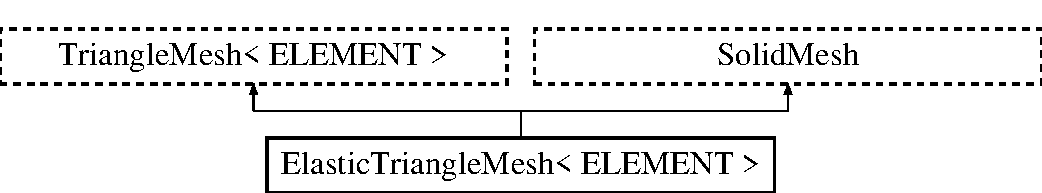
\includegraphics[height=2.000000cm]{classElasticTriangleMesh}
\end{center}
\end{figure}
\subsection*{Public Member Functions}
\begin{DoxyCompactItemize}
\item 
\hyperlink{classElasticTriangleMesh_a4c24e9abbde344d34e1e08fb3319d7b6}{Elastic\+Triangle\+Mesh} (const std\+::string \&node\+\_\+file\+\_\+name, const std\+::string \&element\+\_\+file\+\_\+name, const std\+::string \&poly\+\_\+file\+\_\+name, Time\+Stepper $\ast$time\+\_\+stepper\+\_\+pt=\&Mesh\+::\+Default\+\_\+\+Time\+Stepper)
\begin{DoxyCompactList}\small\item\em Constructor\+: \end{DoxyCompactList}\item 
void \hyperlink{classElasticTriangleMesh_aa83cad3dfdd980f95bf0dab6fd97bf22}{identify\+\_\+boundaries} ()
\begin{DoxyCompactList}\small\item\em Function used to identify the domain boundaries. \end{DoxyCompactList}\item 
virtual \hyperlink{classElasticTriangleMesh_ade80b912f1bb791e5f4fac35abf90504}{$\sim$\+Elastic\+Triangle\+Mesh} ()
\begin{DoxyCompactList}\small\item\em Empty Destructor. \end{DoxyCompactList}\end{DoxyCompactItemize}


\subsection{Detailed Description}
\subsubsection*{template$<$class E\+L\+E\+M\+E\+NT$>$\newline
class Elastic\+Triangle\+Mesh$<$ E\+L\+E\+M\+E\+N\+T $>$}

Triangle-\/based mesh upgraded to become a (pseudo-\/) solid mesh. 

Definition at line 52 of file unstructured\+\_\+two\+\_\+d\+\_\+fluid.\+cc.



\subsection{Constructor \& Destructor Documentation}
\mbox{\Hypertarget{classElasticTriangleMesh_a4c24e9abbde344d34e1e08fb3319d7b6}\label{classElasticTriangleMesh_a4c24e9abbde344d34e1e08fb3319d7b6}} 
\index{Elastic\+Triangle\+Mesh@{Elastic\+Triangle\+Mesh}!Elastic\+Triangle\+Mesh@{Elastic\+Triangle\+Mesh}}
\index{Elastic\+Triangle\+Mesh@{Elastic\+Triangle\+Mesh}!Elastic\+Triangle\+Mesh@{Elastic\+Triangle\+Mesh}}
\subsubsection{\texorpdfstring{Elastic\+Triangle\+Mesh()}{ElasticTriangleMesh()}}
{\footnotesize\ttfamily template$<$class E\+L\+E\+M\+E\+NT$>$ \\
\hyperlink{classElasticTriangleMesh}{Elastic\+Triangle\+Mesh}$<$ E\+L\+E\+M\+E\+NT $>$\+::\hyperlink{classElasticTriangleMesh}{Elastic\+Triangle\+Mesh} (\begin{DoxyParamCaption}\item[{const std\+::string \&}]{node\+\_\+file\+\_\+name,  }\item[{const std\+::string \&}]{element\+\_\+file\+\_\+name,  }\item[{const std\+::string \&}]{poly\+\_\+file\+\_\+name,  }\item[{Time\+Stepper $\ast$}]{time\+\_\+stepper\+\_\+pt = {\ttfamily \&Mesh\+:\+:Default\+\_\+TimeStepper} }\end{DoxyParamCaption})\hspace{0.3cm}{\ttfamily [inline]}}



Constructor\+: 



Definition at line 59 of file unstructured\+\_\+two\+\_\+d\+\_\+fluid.\+cc.

\mbox{\Hypertarget{classElasticTriangleMesh_ade80b912f1bb791e5f4fac35abf90504}\label{classElasticTriangleMesh_ade80b912f1bb791e5f4fac35abf90504}} 
\index{Elastic\+Triangle\+Mesh@{Elastic\+Triangle\+Mesh}!````~Elastic\+Triangle\+Mesh@{$\sim$\+Elastic\+Triangle\+Mesh}}
\index{````~Elastic\+Triangle\+Mesh@{$\sim$\+Elastic\+Triangle\+Mesh}!Elastic\+Triangle\+Mesh@{Elastic\+Triangle\+Mesh}}
\subsubsection{\texorpdfstring{$\sim$\+Elastic\+Triangle\+Mesh()}{~ElasticTriangleMesh()}}
{\footnotesize\ttfamily template$<$class E\+L\+E\+M\+E\+NT$>$ \\
virtual \hyperlink{classElasticTriangleMesh}{Elastic\+Triangle\+Mesh}$<$ E\+L\+E\+M\+E\+NT $>$\+::$\sim$\hyperlink{classElasticTriangleMesh}{Elastic\+Triangle\+Mesh} (\begin{DoxyParamCaption}{ }\end{DoxyParamCaption})\hspace{0.3cm}{\ttfamily [inline]}, {\ttfamily [virtual]}}



Empty Destructor. 



Definition at line 114 of file unstructured\+\_\+two\+\_\+d\+\_\+fluid.\+cc.



\subsection{Member Function Documentation}
\mbox{\Hypertarget{classElasticTriangleMesh_aa83cad3dfdd980f95bf0dab6fd97bf22}\label{classElasticTriangleMesh_aa83cad3dfdd980f95bf0dab6fd97bf22}} 
\index{Elastic\+Triangle\+Mesh@{Elastic\+Triangle\+Mesh}!identify\+\_\+boundaries@{identify\+\_\+boundaries}}
\index{identify\+\_\+boundaries@{identify\+\_\+boundaries}!Elastic\+Triangle\+Mesh@{Elastic\+Triangle\+Mesh}}
\subsubsection{\texorpdfstring{identify\+\_\+boundaries()}{identify\_boundaries()}}
{\footnotesize\ttfamily template$<$class E\+L\+E\+M\+E\+NT$>$ \\
void \hyperlink{classElasticTriangleMesh}{Elastic\+Triangle\+Mesh}$<$ E\+L\+E\+M\+E\+NT $>$\+::identify\+\_\+boundaries (\begin{DoxyParamCaption}{ }\end{DoxyParamCaption})\hspace{0.3cm}{\ttfamily [inline]}}



Function used to identify the domain boundaries. 



Definition at line 76 of file unstructured\+\_\+two\+\_\+d\+\_\+fluid.\+cc.



The documentation for this class was generated from the following file\+:\begin{DoxyCompactItemize}
\item 
\hyperlink{unstructured__two__d__fluid_8cc}{unstructured\+\_\+two\+\_\+d\+\_\+fluid.\+cc}\end{DoxyCompactItemize}

\hypertarget{classUnstructuredFluidProblem}{}\section{Unstructured\+Fluid\+Problem$<$ E\+L\+E\+M\+E\+NT $>$ Class Template Reference}
\label{classUnstructuredFluidProblem}\index{Unstructured\+Fluid\+Problem$<$ E\+L\+E\+M\+E\+N\+T $>$@{Unstructured\+Fluid\+Problem$<$ E\+L\+E\+M\+E\+N\+T $>$}}


Unstructured fluid problem.  


Inheritance diagram for Unstructured\+Fluid\+Problem$<$ E\+L\+E\+M\+E\+NT $>$\+:\begin{figure}[H]
\begin{center}
\leavevmode
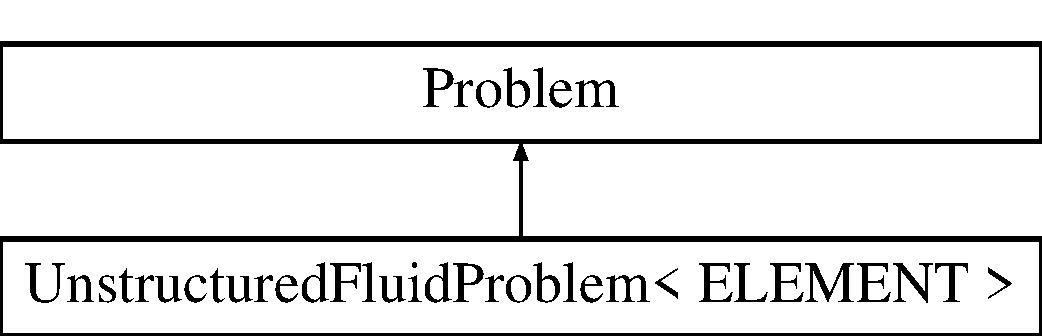
\includegraphics[height=2.000000cm]{classUnstructuredFluidProblem}
\end{center}
\end{figure}
\subsection*{Public Member Functions}
\begin{DoxyCompactItemize}
\item 
\hyperlink{classUnstructuredFluidProblem_a9751f4afac540e148b3d90ae43dd5187}{Unstructured\+Fluid\+Problem} ()
\begin{DoxyCompactList}\small\item\em Constructor\+: \end{DoxyCompactList}\item 
\hyperlink{classUnstructuredFluidProblem_a4d660faa6bae35197a4ea73139ac9963}{$\sim$\+Unstructured\+Fluid\+Problem} ()
\begin{DoxyCompactList}\small\item\em Destructor (empty) \end{DoxyCompactList}\item 
void \hyperlink{classUnstructuredFluidProblem_abcc9f0065665ae5239988b1a812e3f78}{doc\+\_\+solution} (Doc\+Info \&doc\+\_\+info)
\begin{DoxyCompactList}\small\item\em Doc the solution. \end{DoxyCompactList}\item 
unsigned \hyperlink{classUnstructuredFluidProblem_a8afc18327561107094fa94f2918a385f}{nfluid\+\_\+inflow\+\_\+traction\+\_\+boundary} ()
\begin{DoxyCompactList}\small\item\em Return total number of fluid inflow traction boundaries. \end{DoxyCompactList}\item 
unsigned \hyperlink{classUnstructuredFluidProblem_abcaa700f2e0e1b2097e7dc25fe087862}{nfluid\+\_\+outflow\+\_\+traction\+\_\+boundary} ()
\begin{DoxyCompactList}\small\item\em Return total number of fluid outflow traction boundaries. \end{DoxyCompactList}\item 
unsigned \hyperlink{classUnstructuredFluidProblem_ae04e768e915a5e097527cea22558203d}{nfluid\+\_\+traction\+\_\+boundary} ()
\begin{DoxyCompactList}\small\item\em Return total number of fluid outflow traction boundaries. \end{DoxyCompactList}\item 
void \hyperlink{classUnstructuredFluidProblem_ae95f1912572e8a5f0543eab9c0eb2634}{create\+\_\+fluid\+\_\+traction\+\_\+elements} ()
\begin{DoxyCompactList}\small\item\em Create fluid traction elements at inflow. \end{DoxyCompactList}\end{DoxyCompactItemize}
\subsection*{Public Attributes}
\begin{DoxyCompactItemize}
\item 
Tetgen\+Mesh$<$ E\+L\+E\+M\+E\+NT $>$ $\ast$ \hyperlink{classUnstructuredFluidProblem_ade90cb92dd49b9d897ed538b1876b060}{Fluid\+\_\+mesh\+\_\+pt}
\begin{DoxyCompactList}\small\item\em Bulk fluid mesh. \end{DoxyCompactList}\item 
Vector$<$ Mesh $\ast$ $>$ \hyperlink{classUnstructuredFluidProblem_ad2fd96c077dbc69077daaf20a314896c}{Fluid\+\_\+traction\+\_\+mesh\+\_\+pt}
\begin{DoxyCompactList}\small\item\em Meshes of fluid traction elements that apply pressure at in/outflow. \end{DoxyCompactList}\item 
Vector$<$ unsigned $>$ \hyperlink{classUnstructuredFluidProblem_a2923e009bcea7cdbdd7ea5788580a3f8}{Inflow\+\_\+boundary\+\_\+id}
\begin{DoxyCompactList}\small\item\em I\+Ds of fluid mesh boundaries along which inflow boundary conditions are applied. \end{DoxyCompactList}\item 
Vector$<$ unsigned $>$ \hyperlink{classUnstructuredFluidProblem_a9bace139103152045dfe88e3d0163811}{Outflow\+\_\+boundary\+\_\+id}
\begin{DoxyCompactList}\small\item\em I\+Ds of fluid mesh boundaries along which inflow boundary conditions are applied. \end{DoxyCompactList}\end{DoxyCompactItemize}


\subsection{Detailed Description}
\subsubsection*{template$<$class E\+L\+E\+M\+E\+NT$>$\newline
class Unstructured\+Fluid\+Problem$<$ E\+L\+E\+M\+E\+N\+T $>$}

Unstructured fluid problem. 

Definition at line 101 of file unstructured\+\_\+three\+\_\+d\+\_\+fluid.\+cc.



\subsection{Constructor \& Destructor Documentation}
\mbox{\Hypertarget{classUnstructuredFluidProblem_a9751f4afac540e148b3d90ae43dd5187}\label{classUnstructuredFluidProblem_a9751f4afac540e148b3d90ae43dd5187}} 
\index{Unstructured\+Fluid\+Problem@{Unstructured\+Fluid\+Problem}!Unstructured\+Fluid\+Problem@{Unstructured\+Fluid\+Problem}}
\index{Unstructured\+Fluid\+Problem@{Unstructured\+Fluid\+Problem}!Unstructured\+Fluid\+Problem@{Unstructured\+Fluid\+Problem}}
\subsubsection{\texorpdfstring{Unstructured\+Fluid\+Problem()}{UnstructuredFluidProblem()}}
{\footnotesize\ttfamily template$<$class E\+L\+E\+M\+E\+NT $>$ \\
\hyperlink{classUnstructuredFluidProblem}{Unstructured\+Fluid\+Problem}$<$ E\+L\+E\+M\+E\+NT $>$\+::\hyperlink{classUnstructuredFluidProblem}{Unstructured\+Fluid\+Problem} (\begin{DoxyParamCaption}{ }\end{DoxyParamCaption})}



Constructor\+: 

Constructor for unstructured 3D fluid problem. 

Definition at line 160 of file unstructured\+\_\+three\+\_\+d\+\_\+fluid.\+cc.



References Global\+\_\+\+Parameters\+::\+Re.

\mbox{\Hypertarget{classUnstructuredFluidProblem_a4d660faa6bae35197a4ea73139ac9963}\label{classUnstructuredFluidProblem_a4d660faa6bae35197a4ea73139ac9963}} 
\index{Unstructured\+Fluid\+Problem@{Unstructured\+Fluid\+Problem}!````~Unstructured\+Fluid\+Problem@{$\sim$\+Unstructured\+Fluid\+Problem}}
\index{````~Unstructured\+Fluid\+Problem@{$\sim$\+Unstructured\+Fluid\+Problem}!Unstructured\+Fluid\+Problem@{Unstructured\+Fluid\+Problem}}
\subsubsection{\texorpdfstring{$\sim$\+Unstructured\+Fluid\+Problem()}{~UnstructuredFluidProblem()}}
{\footnotesize\ttfamily template$<$class E\+L\+E\+M\+E\+NT$>$ \\
\hyperlink{classUnstructuredFluidProblem}{Unstructured\+Fluid\+Problem}$<$ E\+L\+E\+M\+E\+NT $>$\+::$\sim$\hyperlink{classUnstructuredFluidProblem}{Unstructured\+Fluid\+Problem} (\begin{DoxyParamCaption}{ }\end{DoxyParamCaption})\hspace{0.3cm}{\ttfamily [inline]}}



Destructor (empty) 



Definition at line 110 of file unstructured\+\_\+three\+\_\+d\+\_\+fluid.\+cc.



\subsection{Member Function Documentation}
\mbox{\Hypertarget{classUnstructuredFluidProblem_ae95f1912572e8a5f0543eab9c0eb2634}\label{classUnstructuredFluidProblem_ae95f1912572e8a5f0543eab9c0eb2634}} 
\index{Unstructured\+Fluid\+Problem@{Unstructured\+Fluid\+Problem}!create\+\_\+fluid\+\_\+traction\+\_\+elements@{create\+\_\+fluid\+\_\+traction\+\_\+elements}}
\index{create\+\_\+fluid\+\_\+traction\+\_\+elements@{create\+\_\+fluid\+\_\+traction\+\_\+elements}!Unstructured\+Fluid\+Problem@{Unstructured\+Fluid\+Problem}}
\subsubsection{\texorpdfstring{create\+\_\+fluid\+\_\+traction\+\_\+elements()}{create\_fluid\_traction\_elements()}}
{\footnotesize\ttfamily template$<$class E\+L\+E\+M\+E\+NT $>$ \\
void \hyperlink{classUnstructuredFluidProblem}{Unstructured\+Fluid\+Problem}$<$ E\+L\+E\+M\+E\+NT $>$\+::create\+\_\+fluid\+\_\+traction\+\_\+elements (\begin{DoxyParamCaption}{ }\end{DoxyParamCaption})}



Create fluid traction elements at inflow. 

Create fluid traction elements. 

Definition at line 317 of file unstructured\+\_\+three\+\_\+d\+\_\+fluid.\+cc.



References Global\+\_\+\+Parameters\+::prescribed\+\_\+inflow\+\_\+traction(), and Global\+\_\+\+Parameters\+::prescribed\+\_\+outflow\+\_\+traction().

\mbox{\Hypertarget{classUnstructuredFluidProblem_abcc9f0065665ae5239988b1a812e3f78}\label{classUnstructuredFluidProblem_abcc9f0065665ae5239988b1a812e3f78}} 
\index{Unstructured\+Fluid\+Problem@{Unstructured\+Fluid\+Problem}!doc\+\_\+solution@{doc\+\_\+solution}}
\index{doc\+\_\+solution@{doc\+\_\+solution}!Unstructured\+Fluid\+Problem@{Unstructured\+Fluid\+Problem}}
\subsubsection{\texorpdfstring{doc\+\_\+solution()}{doc\_solution()}}
{\footnotesize\ttfamily template$<$class E\+L\+E\+M\+E\+NT $>$ \\
void \hyperlink{classUnstructuredFluidProblem}{Unstructured\+Fluid\+Problem}$<$ E\+L\+E\+M\+E\+NT $>$\+::doc\+\_\+solution (\begin{DoxyParamCaption}\item[{Doc\+Info \&}]{doc\+\_\+info }\end{DoxyParamCaption})}



Doc the solution. 



Definition at line 388 of file unstructured\+\_\+three\+\_\+d\+\_\+fluid.\+cc.



Referenced by main().

\mbox{\Hypertarget{classUnstructuredFluidProblem_a8afc18327561107094fa94f2918a385f}\label{classUnstructuredFluidProblem_a8afc18327561107094fa94f2918a385f}} 
\index{Unstructured\+Fluid\+Problem@{Unstructured\+Fluid\+Problem}!nfluid\+\_\+inflow\+\_\+traction\+\_\+boundary@{nfluid\+\_\+inflow\+\_\+traction\+\_\+boundary}}
\index{nfluid\+\_\+inflow\+\_\+traction\+\_\+boundary@{nfluid\+\_\+inflow\+\_\+traction\+\_\+boundary}!Unstructured\+Fluid\+Problem@{Unstructured\+Fluid\+Problem}}
\subsubsection{\texorpdfstring{nfluid\+\_\+inflow\+\_\+traction\+\_\+boundary()}{nfluid\_inflow\_traction\_boundary()}}
{\footnotesize\ttfamily template$<$class E\+L\+E\+M\+E\+NT$>$ \\
unsigned \hyperlink{classUnstructuredFluidProblem}{Unstructured\+Fluid\+Problem}$<$ E\+L\+E\+M\+E\+NT $>$\+::nfluid\+\_\+inflow\+\_\+traction\+\_\+boundary (\begin{DoxyParamCaption}{ }\end{DoxyParamCaption})\hspace{0.3cm}{\ttfamily [inline]}}



Return total number of fluid inflow traction boundaries. 



Definition at line 116 of file unstructured\+\_\+three\+\_\+d\+\_\+fluid.\+cc.

\mbox{\Hypertarget{classUnstructuredFluidProblem_abcaa700f2e0e1b2097e7dc25fe087862}\label{classUnstructuredFluidProblem_abcaa700f2e0e1b2097e7dc25fe087862}} 
\index{Unstructured\+Fluid\+Problem@{Unstructured\+Fluid\+Problem}!nfluid\+\_\+outflow\+\_\+traction\+\_\+boundary@{nfluid\+\_\+outflow\+\_\+traction\+\_\+boundary}}
\index{nfluid\+\_\+outflow\+\_\+traction\+\_\+boundary@{nfluid\+\_\+outflow\+\_\+traction\+\_\+boundary}!Unstructured\+Fluid\+Problem@{Unstructured\+Fluid\+Problem}}
\subsubsection{\texorpdfstring{nfluid\+\_\+outflow\+\_\+traction\+\_\+boundary()}{nfluid\_outflow\_traction\_boundary()}}
{\footnotesize\ttfamily template$<$class E\+L\+E\+M\+E\+NT$>$ \\
unsigned \hyperlink{classUnstructuredFluidProblem}{Unstructured\+Fluid\+Problem}$<$ E\+L\+E\+M\+E\+NT $>$\+::nfluid\+\_\+outflow\+\_\+traction\+\_\+boundary (\begin{DoxyParamCaption}{ }\end{DoxyParamCaption})\hspace{0.3cm}{\ttfamily [inline]}}



Return total number of fluid outflow traction boundaries. 



Definition at line 122 of file unstructured\+\_\+three\+\_\+d\+\_\+fluid.\+cc.

\mbox{\Hypertarget{classUnstructuredFluidProblem_ae04e768e915a5e097527cea22558203d}\label{classUnstructuredFluidProblem_ae04e768e915a5e097527cea22558203d}} 
\index{Unstructured\+Fluid\+Problem@{Unstructured\+Fluid\+Problem}!nfluid\+\_\+traction\+\_\+boundary@{nfluid\+\_\+traction\+\_\+boundary}}
\index{nfluid\+\_\+traction\+\_\+boundary@{nfluid\+\_\+traction\+\_\+boundary}!Unstructured\+Fluid\+Problem@{Unstructured\+Fluid\+Problem}}
\subsubsection{\texorpdfstring{nfluid\+\_\+traction\+\_\+boundary()}{nfluid\_traction\_boundary()}}
{\footnotesize\ttfamily template$<$class E\+L\+E\+M\+E\+NT$>$ \\
unsigned \hyperlink{classUnstructuredFluidProblem}{Unstructured\+Fluid\+Problem}$<$ E\+L\+E\+M\+E\+NT $>$\+::nfluid\+\_\+traction\+\_\+boundary (\begin{DoxyParamCaption}{ }\end{DoxyParamCaption})\hspace{0.3cm}{\ttfamily [inline]}}



Return total number of fluid outflow traction boundaries. 



Definition at line 128 of file unstructured\+\_\+three\+\_\+d\+\_\+fluid.\+cc.



\subsection{Member Data Documentation}
\mbox{\Hypertarget{classUnstructuredFluidProblem_ade90cb92dd49b9d897ed538b1876b060}\label{classUnstructuredFluidProblem_ade90cb92dd49b9d897ed538b1876b060}} 
\index{Unstructured\+Fluid\+Problem@{Unstructured\+Fluid\+Problem}!Fluid\+\_\+mesh\+\_\+pt@{Fluid\+\_\+mesh\+\_\+pt}}
\index{Fluid\+\_\+mesh\+\_\+pt@{Fluid\+\_\+mesh\+\_\+pt}!Unstructured\+Fluid\+Problem@{Unstructured\+Fluid\+Problem}}
\subsubsection{\texorpdfstring{Fluid\+\_\+mesh\+\_\+pt}{Fluid\_mesh\_pt}}
{\footnotesize\ttfamily template$<$class E\+L\+E\+M\+E\+NT$>$ \\
Tetgen\+Mesh$<$E\+L\+E\+M\+E\+NT$>$$\ast$ \hyperlink{classUnstructuredFluidProblem}{Unstructured\+Fluid\+Problem}$<$ E\+L\+E\+M\+E\+NT $>$\+::Fluid\+\_\+mesh\+\_\+pt}



Bulk fluid mesh. 



Definition at line 139 of file unstructured\+\_\+three\+\_\+d\+\_\+fluid.\+cc.

\mbox{\Hypertarget{classUnstructuredFluidProblem_ad2fd96c077dbc69077daaf20a314896c}\label{classUnstructuredFluidProblem_ad2fd96c077dbc69077daaf20a314896c}} 
\index{Unstructured\+Fluid\+Problem@{Unstructured\+Fluid\+Problem}!Fluid\+\_\+traction\+\_\+mesh\+\_\+pt@{Fluid\+\_\+traction\+\_\+mesh\+\_\+pt}}
\index{Fluid\+\_\+traction\+\_\+mesh\+\_\+pt@{Fluid\+\_\+traction\+\_\+mesh\+\_\+pt}!Unstructured\+Fluid\+Problem@{Unstructured\+Fluid\+Problem}}
\subsubsection{\texorpdfstring{Fluid\+\_\+traction\+\_\+mesh\+\_\+pt}{Fluid\_traction\_mesh\_pt}}
{\footnotesize\ttfamily template$<$class E\+L\+E\+M\+E\+NT$>$ \\
Vector$<$Mesh$\ast$$>$ \hyperlink{classUnstructuredFluidProblem}{Unstructured\+Fluid\+Problem}$<$ E\+L\+E\+M\+E\+NT $>$\+::Fluid\+\_\+traction\+\_\+mesh\+\_\+pt}



Meshes of fluid traction elements that apply pressure at in/outflow. 



Definition at line 142 of file unstructured\+\_\+three\+\_\+d\+\_\+fluid.\+cc.

\mbox{\Hypertarget{classUnstructuredFluidProblem_a2923e009bcea7cdbdd7ea5788580a3f8}\label{classUnstructuredFluidProblem_a2923e009bcea7cdbdd7ea5788580a3f8}} 
\index{Unstructured\+Fluid\+Problem@{Unstructured\+Fluid\+Problem}!Inflow\+\_\+boundary\+\_\+id@{Inflow\+\_\+boundary\+\_\+id}}
\index{Inflow\+\_\+boundary\+\_\+id@{Inflow\+\_\+boundary\+\_\+id}!Unstructured\+Fluid\+Problem@{Unstructured\+Fluid\+Problem}}
\subsubsection{\texorpdfstring{Inflow\+\_\+boundary\+\_\+id}{Inflow\_boundary\_id}}
{\footnotesize\ttfamily template$<$class E\+L\+E\+M\+E\+NT$>$ \\
Vector$<$unsigned$>$ \hyperlink{classUnstructuredFluidProblem}{Unstructured\+Fluid\+Problem}$<$ E\+L\+E\+M\+E\+NT $>$\+::Inflow\+\_\+boundary\+\_\+id}



I\+Ds of fluid mesh boundaries along which inflow boundary conditions are applied. 



Definition at line 146 of file unstructured\+\_\+three\+\_\+d\+\_\+fluid.\+cc.

\mbox{\Hypertarget{classUnstructuredFluidProblem_a9bace139103152045dfe88e3d0163811}\label{classUnstructuredFluidProblem_a9bace139103152045dfe88e3d0163811}} 
\index{Unstructured\+Fluid\+Problem@{Unstructured\+Fluid\+Problem}!Outflow\+\_\+boundary\+\_\+id@{Outflow\+\_\+boundary\+\_\+id}}
\index{Outflow\+\_\+boundary\+\_\+id@{Outflow\+\_\+boundary\+\_\+id}!Unstructured\+Fluid\+Problem@{Unstructured\+Fluid\+Problem}}
\subsubsection{\texorpdfstring{Outflow\+\_\+boundary\+\_\+id}{Outflow\_boundary\_id}}
{\footnotesize\ttfamily template$<$class E\+L\+E\+M\+E\+NT$>$ \\
Vector$<$unsigned$>$ \hyperlink{classUnstructuredFluidProblem}{Unstructured\+Fluid\+Problem}$<$ E\+L\+E\+M\+E\+NT $>$\+::Outflow\+\_\+boundary\+\_\+id}



I\+Ds of fluid mesh boundaries along which inflow boundary conditions are applied. 



Definition at line 150 of file unstructured\+\_\+three\+\_\+d\+\_\+fluid.\+cc.



The documentation for this class was generated from the following file\+:\begin{DoxyCompactItemize}
\item 
\hyperlink{unstructured__three__d__fluid_8cc}{unstructured\+\_\+three\+\_\+d\+\_\+fluid.\+cc}\end{DoxyCompactItemize}

\chapter{File Documentation}
\hypertarget{unstructured__fluid_8txt__doxygenified_8h}{}\section{unstructured\+\_\+fluid.\+txt\+\_\+doxygenified.\+h File Reference}
\label{unstructured__fluid_8txt__doxygenified_8h}\index{unstructured\+\_\+fluid.\+txt\+\_\+doxygenified.\+h@{unstructured\+\_\+fluid.\+txt\+\_\+doxygenified.\+h}}

\hypertarget{unstructured__two__d__fluid_8cc}{}\section{unstructured\+\_\+two\+\_\+d\+\_\+fluid.\+cc File Reference}
\label{unstructured__two__d__fluid_8cc}\index{unstructured\+\_\+two\+\_\+d\+\_\+fluid.\+cc@{unstructured\+\_\+two\+\_\+d\+\_\+fluid.\+cc}}
\subsection*{Classes}
\begin{DoxyCompactItemize}
\item 
class \hyperlink{classElasticTriangleMesh}{Elastic\+Triangle\+Mesh$<$ E\+L\+E\+M\+E\+N\+T $>$}
\begin{DoxyCompactList}\small\item\em Triangle-\/based mesh upgraded to become a (pseudo-\/) solid mesh. \end{DoxyCompactList}\item 
class \hyperlink{classUnstructuredFluidProblem}{Unstructured\+Fluid\+Problem$<$ E\+L\+E\+M\+E\+N\+T $>$}
\begin{DoxyCompactList}\small\item\em Unstructured fluid problem. \end{DoxyCompactList}\end{DoxyCompactItemize}
\subsection*{Namespaces}
\begin{DoxyCompactItemize}
\item 
 \hyperlink{namespaceGlobal__Physical__Variables}{Global\+\_\+\+Physical\+\_\+\+Variables}
\begin{DoxyCompactList}\small\item\em Namespace for physical parameters. \end{DoxyCompactList}\end{DoxyCompactItemize}
\subsection*{Functions}
\begin{DoxyCompactItemize}
\item 
int \hyperlink{unstructured__two__d__fluid_8cc_ae66f6b31b5ad750f1fe042a706a4e3d4}{main} ()
\begin{DoxyCompactList}\small\item\em Driver for unstructured fluid test problem. \end{DoxyCompactList}\end{DoxyCompactItemize}
\subsection*{Variables}
\begin{DoxyCompactItemize}
\item 
double \hyperlink{namespaceGlobal__Physical__Variables_ab814e627d2eb5bc50318879d19ab16b9}{Global\+\_\+\+Physical\+\_\+\+Variables\+::\+Re} =0.\+0
\begin{DoxyCompactList}\small\item\em Reynolds number. \end{DoxyCompactList}\item 
double \hyperlink{namespaceGlobal__Physical__Variables_a3962c36313826b19f216f6bbbdd6a477}{Global\+\_\+\+Physical\+\_\+\+Variables\+::\+Nu} =0.\+3
\begin{DoxyCompactList}\small\item\em Pseudo-\/solid Poisson ratio. \end{DoxyCompactList}\item 
Constitutive\+Law $\ast$ \hyperlink{namespaceGlobal__Physical__Variables_a2a37fb040c832ee7a086bb13bb02a100}{Global\+\_\+\+Physical\+\_\+\+Variables\+::\+Constitutive\+\_\+law\+\_\+pt} =0
\begin{DoxyCompactList}\small\item\em Constitutive law used to determine the mesh deformation. \end{DoxyCompactList}\end{DoxyCompactItemize}


\subsection{Function Documentation}
\mbox{\Hypertarget{unstructured__two__d__fluid_8cc_ae66f6b31b5ad750f1fe042a706a4e3d4}\label{unstructured__two__d__fluid_8cc_ae66f6b31b5ad750f1fe042a706a4e3d4}} 
\index{unstructured\+\_\+two\+\_\+d\+\_\+fluid.\+cc@{unstructured\+\_\+two\+\_\+d\+\_\+fluid.\+cc}!main@{main}}
\index{main@{main}!unstructured\+\_\+two\+\_\+d\+\_\+fluid.\+cc@{unstructured\+\_\+two\+\_\+d\+\_\+fluid.\+cc}}
\subsubsection{\texorpdfstring{main()}{main()}}
{\footnotesize\ttfamily int main (\begin{DoxyParamCaption}{ }\end{DoxyParamCaption})}



Driver for unstructured fluid test problem. 



Definition at line 374 of file unstructured\+\_\+two\+\_\+d\+\_\+fluid.\+cc.



References Global\+\_\+\+Physical\+\_\+\+Variables\+::\+Constitutive\+\_\+law\+\_\+pt, Unstructured\+Fluid\+Problem$<$ E\+L\+E\+M\+E\+N\+T $>$\+::fluid\+\_\+mesh\+\_\+pt(), Global\+\_\+\+Physical\+\_\+\+Variables\+::\+Nu, and Global\+\_\+\+Physical\+\_\+\+Variables\+::\+Re.


%--- End generated contents ---

% Index
\backmatter
\newpage
\phantomsection
\clearemptydoublepage
\addcontentsline{toc}{chapter}{Index}
\printindex

